\published{Journal of Geophysics and Engineering, 12, 12-25, (2015)}

\title{Random noise attenuation by a selective hybrid approach using f-x empirical mode decomposition}
\renewcommand{\thefootnote}{\fnsymbol{footnote}}

\author{Yangkang Chen\footnotemark[1], Shuwei Gan\footnotemark[2], Tingting Liu\footnotemark[2], Jiang Yuan\footnotemark[2], Yizhuo Zhang\footnotemark[3] and Zhaoyu Jin\footnotemark[3]}


\address{
\footnotemark[1]Bureau of Economic Geology \\
John A. and Katherine G. Jackson School of Geosciences \\
The University of Texas at Austin \\
University Station, Box X \\
Austin, TX 78713-8924 \\

\footnotemark[2] State Key Laboratory of Petroleum Resources and Prospecting \\
China University of Petroleum \\
Fuxue Road 18th\\
Beijing, China, 102200 \\

\footnotemark[3] Grant Institute, The King's Buildings, West Mains Road \\
University of Edinburgh \\
Edinburgh,UK, EH9 3JW \\
}

\lefthead{Chen et al.}
\righthead{Selective hybrid $f-x$ EMD}

\maketitle

\begin{abstract}
Empirical mode decomposition (EMD) becomes attractive recently for random noise attenuation because of its convenient implementation and ability in dealing with non-stationary seismic data. In this paper, we summarize the existing use of EMD in seismic data denoising and introduce a general hybrid scheme which combines $f-x$ EMD with a dipping-events retrieving operator. The novel hybrid scheme can achieve a better denoising performance compared with the conventional $f-x$ EMD and selected dipping event retriever. We demonstrate the strong horizontal-preservation capability of $f-x$ EMD that makes the EMD based hybrid approach attractive. When $f-x$ EMD is applied to a seismic profile, all the horizontal events will be preserved, while leaving few dipping events and random noise in the noise section, which can be dealt with easily by applying a dipping-events retrieving operator to a specific region for preserving the useful dipping signal. This type of incomplete hybrid approach is termed as \textit{selective hybrid} approach. Two synthetic and one post-stack field data examples demonstrate a better performance of the proposed approach.
\end{abstract}

\section{Introduction}
The rapid development of the exploration for unconventional resource raise a higher demand for random noise attenuation of pre- and post-stack seismic profile because of the higher demand for processing noisy land seismic data. Existing denoising techniques can be divided into four categories. The first is based on the predictive property of useful signal, such as predictive filtering \cite[]{canales,abma1995,yanghua1999,guochang2012,yangkang20132}. \old{This type}\new{These types} of methods can achieve good result for linear events but may fail in handling complex or hyperbolic events. The way to deal with this linear-events dependence limitation is to use small local windows. However, different window size will results in different denoising effects and window size is actually data dependent. Thus, localized versions of the first type of methods with small processing windows are often hard to be implemented in practice. The second is based on statistical properties of seismic data, such as mean filter \cite[]{nlm}, median filter \cite[]{yangkang2014svmf,yangkang2014nmo}. \old{This type}\new{These types} of methods are often used to attenuate specific types of random noise. For example, a mean filter is only effective to attenuate highly Gaussian white noise, and a median filter can only remove spike-like random noise with excellent performance. The third is based on extracting the principal components of seismic data, such as singular spectrum analysis (SSA) \cite[]{mssa,yangkang2014eage1}, and $f-x$ EMD \cite[]{bekara,yangkang2014emdsum}. For these methods, first several components are selected to represent the main useful signals. \old{This type}\new{These types} of methods are based on a pre-known mode or rank of the seismic data. However, for complex seismic data, the mode or rank is hard to select, and for curved events, the rank or mode tends to be high and thus will involve a serious rank-mixing problem. The fourth is based on a transformed domain thresholding strategy, such as \new{the papers of} \cite{wavelet,curvelet,seislet,yangkang20142}. The transformed domain thresholding methods can be easily implemented, however, they require strictly that the transformed domain is sparse. For complicated seismic profiles, seldom sparsity-promoting transform can obtain an ideal sparse representation, which limits the use of the fourth type of methods.  

\cite{emd} proposed empirical mode decomposition (EMD) to prepare stable input for the Hilbert Transform. 
The essence of EMD is to stabilize a non-stationary signal. That is, to decompose a signal into a series of intrinsic mode functions (IMF). Each IMF has a relatively local-constant frequency. The frequency of each IMF decreases according to the separation sequence of each IMF.  EMD is a breakthrough in the analysis of linear and stable spectra. It adaptively separates non-linear and non-stationary signals, which are features of seismic data, into different frequency ranges. \cite{bekara} applied $f-x$ EMD to attenuation of random noise, which was demonstrated to perform better than $f-x$ predictive filtering.  Recently a type of hybrid denoising approaches using EMD is becoming attractive. \cite{chenwei2012} proposed to combine  EEMD, an enhanced version of EMD, with wavelet domain thresholding, to obtained a better denoised result. Similarly, \cite{lieqian2013} combined $f-x$ EMD with curvelet domain thresholding, and also obtained better results compared with individual denoising performances. \cite{yangkang20132} noticed the problem of $f-x$ EMD in dealing with complex structure and solve it by introducing $f-x$ empirical mode decomposition predictive filtering (EMDPF), which combine the advantage of both $f-x$ EMD and $f-x$ predictive filtering.  A combination between $f-x$ EMD and one other random noise attenuation approach is becoming more and more attractive because of the special property of $f-x$ EMD in preserving horizontal events.

In this paper, we demonstrate the horizontal-preservation ability of $f-x$ EMD and show the problem of $f-x$ EMD in handling with dipping events. We summarize the connections between the currently existing EMD based denoising approaches and generalize the methods into a general hybrid framework. The principle is to first separate the events in a seismic profile into two parts: horizontal events and dipping events, and then denoise them individually. Because of the strong horizontal-preservation ability of $f-x$ EMD, the horizontal events can be effectively denoised and fully preserved. The dipping events can be preserved by applying a dipping-events retriever that can denoise and preserve dipping events effectively. The hybrid approach solves the problem of $f-x$ EMD in preserving the dipping events, and improve the dipping-event retrieving operator by obtaining cleaner denoised horizontal events. 

Considering that in most seismic profiles, dipping events or steeply dipping events takes up a small percent of the total signals, a \textit{selective hybrid} strategy is also proposed. In the selective hybrid framework, only specific processing windows are processed twice by two different denoising operators, which can helps to maximize the effectiveness of $f-x$ EMD and the whole processing efficiency. Instead of combining $f-x$ EMD with $f-x$ predictive filtering, wavelet thresholding or curvelet thresholding, a novel hybrid approach is to combine $f-x$ EMD with $f-x$ singular spectrum analysis (SSA). Both synthetic and field data examples demonstrate the superior property of the proposed approach.

\section{Background theory}
\subsection{EMD}
The aim of empirical mode decomposition (EMD) is to empirically decompose a non-stationary signal into a finite set of sub-signals, which are termed as intrinsic mode functions (IMF) and are considered to be stationary. The IMFs satisfy two conditions: (1) in the whole data set, the number of extrema and the number of zero crossings must either \new{be} equal or differ at most by one; and (2) at any point, the mean value of the envelope\new{s} defined by the local maxima and \old{the envelope defined by} the local minima is \new{reasonably close to} zero \cite[]{emd}.

Provided that $s(t)$, $c_n(t)$, $r(t)$, and $N$ denote the original non-stationary signal, the separated IMFs, the residual and the number of IMFs, respectively, EMD can be expressed as:
\begin{equation}
\label{eq:emd}
s(t)=\sum_{n=1}^{N}c_n(t)+r(t).
\end{equation}
For a non-stationary signal $s(t)$, using equation \ref{eq:emd}, we get a finite set of sub-signals $c_n(t)$,($n=1,2,\cdots,N$). 

A special property of EMD is that the IMFs represent different oscillations embedded in the data, where the mean frequency for each sub-signal $c_n(t)$ decreases with IMF order increasing. 

Figures \ref{fig:s-sf} and \ref{fig:Imf} give a example of EMD for a non-stationary signal. Figure \ref{fig:s-sf} shows a non-stationary signal and its corresponding instantaneous frequency, which is similar to that used by \cite{herrera2013}. From the instantaneous frequency we can see that the signal can be divided into four temporal regions. From 0 s - 4 s, the signal is composed of two frequency components corresponding to 5 Hz and 15 Hz. From 4 s - 6 s, the signal is composed of three frequency components corresponding to 5 Hz, 15 Hz, and 34 Hz, respectively. From 6 s- 7.8 s, the signal is composed of two frequency components corresponding to 10 Hz and 34 Hz. The last part from 7.8 s to 10 s is a monotonic signal, whose frequency is 10 Hz. Figure \ref{fig:Imf} \old{shown}\new{shows} the separated signal component using EMD. The separated components are consistent with the instantaneous frequency map as shown in Figure \ref{fig:s-sf}. Each individual frequency components have been separated out, with negligible edge effects and residual.

\inputdir{nonstat}

\plot{s-sf}{width=\textwidth}{Non-stationary signal and its instantaneous frequency. Up: Non-stationary signal. Down: Corresponding instantaneous frequency.}

\plot{Imf}{width=\textwidth}{EMD separated signal. From up to down: first IMF, second IMF, third IMF, and the residual.}

\subsection{$f-x$ EMD}
$f-x$ EMD was proposed by \cite{bekara} to attenuate random noise. They applied EMD on
each frequency slice in the $f-x$ domain, and remove the first IMF,
which mainly represent the higher wavenumber components. The methodology can be summarized as:

\begin{equation}
\label{eq:fxemd}
\begin{split}
\hat{s}(m,t) &= \mathcal{F}^{-1}\left(\sum_{n=2}^{N}C_n(m,w)\right), \\
\mathcal{F} d(m,t)  &= \sum_{n=1}^{N} C_n(m,w),
\end{split}
\end{equation}
where $\hat{s}(m,t)$ and $d(m,t)$ denote the estimated signal and acquired noisy signal, respectively. $\mathcal{F}$ and $\mathcal{F}^{-1}$ denote the forward and inverse Fourier transforms along the time axis, respectively. $C_n$ denotes the $n$th EMD decomposed component. $w$ denotes frequency. However, a problem occurs when applying $f-x$
EMD, because the dipping events will also be removed.
This problem occurs because, for many data sets, the random noise and any steeply dipping coherent
energy make a significantly larger contribution to the high-wavenumber energy in the $f-x$
domain than any desired signal \cite[]{bekara}.

\subsection{$f-x$ SSA}
Matrix completion via $f-x$ domain singular spectrum analysis (SSA) can handle complex dipping events well by extracting the first several eigen components after SVD for each frequency slice. 
Considering 2D seismic data acquired on a regular grid $D(m,w)$, $m=1,\cdots, M$, where $M$ denotes the number of traces in the spatial dimension.
The Hankel matrix for each frequency slice $D(m,w)$ is constructed as:
\begin{equation}
\label{eq:mssa}
\mathbf{H}=\left(\begin{array}{cccc}
D(1,w) & D(2,w) & \cdots &D(K,w) \\
D(2,w) & D(3,w)  &\cdots &D(K+1,w) \\
\vdots & \vdots &\ddots &\vdots \\
D(L,w)&D(L+1,w) &\cdots&D(M,w)
\end{array}
\right),
\end{equation}
where $L=\lfloor\frac{M}{2}\rfloor+1$ and $K=M-L+1$,\old{ and} $\lfloor\rfloor$ denotes the integer part of its argument\new{, $w$ denotes frequency}. 
It can be proved that if the processing window contains $k$ plane waves of independent dips, then the Hankel matrix $\mathbf{H}$ is rank k. The added random noise will increase the rank of matrix $\mathbf{H}$. It's natural that the random noise can be removed by rank reduction for $\mathbf{H}$ \cite[]{mssa}. A singular value decomposition (SVD) is applied to the Hankel matrix in order to select the first several eigen components that correspond to the first several singular values. The $f-x$ SSA approach is based on a pre-known rank of the seismic data. However, for complex seismic data, the rank is hard to select, and for curved events, the rank tends to be high and thus will involve a serious rank-mixing problem. The simpler the seismic profile is, the easier it is to choose the predefined matrix rank because the rank-mixing problem is less serious. \cite{sanyi2011} \old{come}\new{came up} up a way to simplify $f-x$ SSA. They applied $f-x$ SSA in a local version to reduce the complexity of seismic events in order to make the rank of the aforementioned Hankel matrix lower.




\section{Horizontal preservation and dipping removal for $f-x$ EMD}
\cite{bekara} proposed to use $f-x$ EMD to remove random and coherent noise in seismic profiles. Their strategy is based on the fact that $f-x$ EMD can preserve the horizontal events, which can be seen as useful reflection signals, and can remove un-horizontal signals, which can be seen as a combination of random noise and coherent dipping noise. However, for those seismic profiles with complex structures, the strategy does not hold because of the severe loss for dipping useful signals. In this section, we will analyze and show the horizontal-preservation and dipping-removal effects for $f-x$ EMD. 

The process of EMD is to gradually remove the stable oscillations embedded in the original signal and obtain a monotonic and smooth residual or trend at last. When it is applied to the seismic profile in each frequency slice along the spatial direction in the $f-x$ domain, the spatially-variant components, usually denoting the dipping events and random noise, will be gradually removed and the spatially-invariant components will be obtained as the residual at last. The small-dip-angle or exactly-horizontal events seismic profile can be considered as spatially invariant or spatially monotonic, thus they can be safely preserved no matter how many IMFs are removed in the frequency-slice decomposition process. On the other hand, the more IMFs are removed, the heavier damage of the dipping events will be caused.

Figure \ref{fig:flat-clean,flat-noise,flat-noisy,flat-denoised,flat-noise1} shows a demonstration of $f-x$ EMD for a flat-event synthetic section. In each panel, the upper graph is the real part of 20 Hz frequency slice, and the down profile is the corresponding synthetic section. The clean data, added Gaussian white noise, and noisy data are shown in Figures \ref{fig:flat-clean}, \ref{fig:flat-noise} and \ref{fig:flat-noisy}, respectively. From the 20 Hz frequency slice we can see the flat event has zero spatial frequency. After $f-x$ EMD with 4 IMFs removed in each frequency slices, the denoised section is very clean, with the corresponding 20 Hz frequency slice nearly constant, the perfect denoising effect can be verified by looking at the removed noise section, where no coherent signal is found and the spectrum is nearly the same as that of the original added Gaussian white noise section. 

The perfect denoising performance does not hold for a dipping-event synthetic section, which is shown in Figure \ref{fig:dip-clean,dip-noise,dip-noisy,dip-denoised1,dip-denoised2,dip-denoised3,dip-noise1,dip-noise2,dip-noise3}. According to the spectrum of the clean dipping event shown in Figure \ref{fig:dip-clean}, we know that a dipping event corresponds to a sine curve in the 20 Hz slice of the frequency domain. In this case, denoising performances corresponding to different number of removed IMFs are compared. Figures \ref{fig:dip-denoised1}, \ref{fig:dip-denoised2} and \ref{fig:dip-denoised3} shows the denoised section by removing 1, 2 and 3 IMFs, respectively. Figures \ref{fig:dip-noise1}, \ref{fig:dip-noise2} and \ref{fig:dip-noise3} are corresponding noise sections. It's obvious that by removing only 1 IMF, the useful dipping signal has been harmed to a large extent. After removing 2 IMFs, most of the useful energy has been removed. Removing 3 IMFs removes totally the dipping event from the data section and the sine curve from the spectrum graph. For field seismic data that contains complex subsurface structure, $f-x$ EMD \old{can not}\new{cannot} be effective, which becomes its biggest issue.

\inputdir{fxemddemo}

\multiplot{5}{flat-clean,flat-noise,flat-noisy,flat-denoised,flat-noise1}{width=0.2600\textwidth,height=0.2801\textwidth}{A demonstration of $f-x$ EMD for a flat-event section. In each panel, the upper graph corresponds to 20 Hz frequency slice (real part), the down profile is the corresponding synthetic section. Four IMFs are removed during $f-x$ EMD. (a) For the clean data. (b) For the added noise section. (c) For the noisy data. (d) For the denoised data. (e) For the separated noise section.}

\multiplot{9}{dip-clean,dip-noise,dip-noisy,dip-denoised1,dip-denoised2,dip-denoised3,dip-noise1,dip-noise2,dip-noise3}{width=0.2600\textwidth,height=0.2801\textwidth}{A demonstration of $f-x$ EMD for a dipping-event. In each panel, the upper graph corresponds to 20 Hz frequency slice (real part), the down profile is the corresponding synthetic section. (a) For the clean data. (b) For the added noise section. (c) For the noisy data. (d) For the denoised data by removing 1 IMF. (e) For the denoised data by removing 2 IMFs. (f) For the denoised data by removing 3 IMFs. (g) For the separated noise section corresponding to (d).  (h) For the separated noise section corresponding to (e). (i) For the separated noise section corresponding to (f).}


%For a noisy synthetic section with relatively small number of plane waves like the one shown in Figure \ref{fig:dip-noisy}, $f-x$ SSA can be especially effective, because the useful signal can be captured with a low rank extraction from the Hankel matrix without including too much noise components. Figure \ref{fig:dip-mssa_denoised,dip-mssa_noise} shows the denoised results using $f-x$ SSA for the noisy dipping-event section shown in Figure \ref{fig:dip-noisy}. The spectrum of the denoised section is much similar to that of the original clean data, and the noise section doesn't contain any coherent signal, which demonstrates the effective performance of $f-x$ SSA. The rank of the Hankel matrix \ref{eq:mssa} for this case is reduced to 1.

\inputdir{fxmssademo}

\multiplot{2}{dip-mssa-denoised,dip-mssa-noise}{width=0.2600\textwidth,height=0.2801\textwidth}{A demonstration of $f-x$ \old{M}SSA for a dipping-event section shown in Figure \ref{fig:dip-noisy}. In each panel, the upper graph corresponds to 20 Hz frequency slice (real part), the down profile is the corresponding synthetic section.  (a) Denoised section. (b) Separated noise section. }


%Considering 2D spatial data acquired on a regular grid $S(m,n,w)$, $m=1,\cdots, N_y$, $n=1,\cdots,N_x$. The signal at a given monochromatic frequency can be represented by the following matrix \cite[]{mssa}:
%\begin{equation}
%\label{eq:mssa1}
%\mathbf{S}=\left(\begin{array}{cccc}
%\mathbf{S}(1,1) & \mathbf{S}(1,2) & \cdots &\mathbf{S}(1,N_x) \\
%\mathbf{S}(2,1) & \mathbf{S}(2,2)  &\cdots &\mathbf{S}(2,N_x) \\
%\vdots & \vdots &\ddots &\vdots \\
%\mathbf{S}(N_y,1)&\mathbf{S}(N_y,2) &\cdots&\mathbf{S}(N_y,N_x)
%\end{array}
%\right),
%\end{equation}
%where $N_x$ and $N_y$ denotes the number of traces in the $x$ and $y$ dimensions, respectively. Here, the argument $w$ has been omitted for concisity. 

%The a Hankel matrix for each row of $\mathbf{S}$ is constructed as:
%\begin{equation}
%\label{eq:mssa2}
%\mathbf{H}_j=\left(\begin{array}{cccc}
%\mathbf{S}(j,1) & \mathbf{S}(j,2) & \cdots &\mathbf{S}(j,K_x) \\
%\mathbf{S}(j,2) & \mathbf{S}(j,3)  &\cdots &\mathbf{S}(j,K_x+1) \\
%\vdots & \vdots &\ddots &\vdots \\
%\mathbf{S}(j,L_x)&\mathbf{S}(j,L_x+1) &\cdots&\mathbf{S}(j,N_x)
%\end{array}
%\right),
%\end{equation}
%where $L_x=\lfloor\frac{N_x}{2}\rfloor+1$ and $K_x=N_x-L_x+1$, and $\lfloor\cdot\rfloor$ denotes the interger part of its argument. Next, we add the $y$ dimension to the analysis by constructing a block Hankel matrix composed of $\mathbf{R}_j$:
%\begin{equation}
%\label{eq:mssa3}
%\mathbf{H}=\left(\begin{array}{cccc}
%\mathbf{H}_1 & \mathbf{H}_2 & \cdots &\mathbf{H}_{K_y}\\
%\mathbf{H}_2 & \mathbf{H}_3  &\cdots &\mathbf{H}_{K_y+1} \\
%\vdots & \vdots &\ddots &\vdots \\
%\mathbf{H}_{L_y}&\mathbf{H}_{L_y+1} &\cdots&\mathbf{R}_{N_y}
%\end{array}
%\right),
%\end{equation} 
%where $L_y=\lfloor\frac{N_y}{2}\rfloor+1$ and $K_y=N_y-L_y+1$.

%It can be proved that if the processing window contains $k$ plane waves of independent dips, then the block Hankel matrix $\mathbf{H}$ is rank k. The added random noise will increase the rank of matrix $\mathbf{H}$. It's natural that the random noise can be removed by rank reduction for $\mathbf{H}$.

\section{Hybrid denoising approach}
Provided that the noisy data $\mathbf{d}$ is composed of the clean data $\mathbf{s}$ and noise $\mathbf{n}$, $f-x$ EMD can get a denoised section with all the horizontal events $\hat{\mathbf{s}}_{h}$, while leaving the dipping events in the noise section: 
\begin{equation}
\label{eq:emd1}
\begin{split}
\hat{\mathbf{s}}_{h} &\approx \mathbf{E}[\mathbf{d}], \\
\mathbf{s}_{d} + \mathbf{n} &\approx \mathbf{d}- \mathbf{E}[\mathbf{d}].
\end{split}
\end{equation}
Here, $\mathbf{E}$ denotes the noise attenuation operator by $f-x$ EMD, $\mathbf{s}_d$ denotes the true dipping events, and $\mathbf{n}$ denotes random noise in the original seismic section.

We can retrieve the useful dipping events by applying another denoising operator onto the noise section,
\begin{equation}
\label{eq:emd3}
\hat{\mathbf{s}}_d \approx \mathbf{P}[ \mathbf{d}- \mathbf{E}[\mathbf{d}] ],
\end{equation}
where $\mathbf{P}$ denotes a denoising operator which estimate the lost dipping events from the initial noise section, and $\hat{\mathbf{s}}_d$ denotes the estimated dipping events. The final denoised section $\hat{\mathbf{s}}$ is given by the summation of the horizontal and dipping signal section:
\begin{equation}
\label{eq:emd4}
\hat{\mathbf{s}} = \hat{\mathbf{s}}_h + \hat{\mathbf{s}}_d \approx \mathbf{E}[\mathbf{d}] + \mathbf{P}[ \mathbf{d}- \mathbf{E}[\mathbf{d}] ].
\end{equation}

The denoising operator $\mathbf{P}$ in equation \ref{eq:emd3} can be chosen as $f-x$ predictive filtering \cite[]{yangkang20132}, wavelet transform \cite[]{chenwei2012}, or curvelet transform \cite[]{lieqian2013}. Thus, equation \ref{eq:emd3} becomes a general framework for all those $f-x$ EMD based random noise attenuation approaches. To extend its generality, we propose to use $f-x$ SSA \cite[]{mssa} as $\mathbf{P}$ in this paper.

The effectiveness of the novel approach can be ascribed to the strong horizontal-preservation ability of $f-x$ EMD. When most of the useful horizontal energy is preserved after $f-x$ EMD, we turn to deal with less number of plane-wave components in the noise section, which is much easier because less signal components usually correspond to a more strict control over the random noise, e.g., smaller prediction length in $f-x$ predictive filtering \cite[]{canales} and lower rank for extracting useful components in $f-x$ SSA \cite[]{mssa}. For example, lower rank corresponds to less-serious rank-mixing problem, that is , less amount of random noise can be leaked into the denoised section.


\section{Selective hybrid denoising approach}

%The effectiveness of the novel approach can be ascribed to the strong ability of $f-x$ EMD in preserving horizontal events. Since the horizontal events correspond to zero spatial frequency, the useful horizontal components becomes the residual for the EMD process for each frequency slice, which is preserved at last. 

Considering that in most seismic profiles, dipping events or steeply dipping events takes up a small percent of the total signals, thus the dipping-events retrieving process shown in equation \ref{eq:emd3} in the above proposed hybrid approach doesn't need to be applied in each processing window for the whole seismic profile. Instead, we can select specific processing window for hybrid processing, this type of incomplete hybrid approach is termed as \textit{selective hybrid} approach.
The detailed algorithmic steps of the selective hybrid approach for random noise attenuation using $f-x$ EMD are shown below:
\begin{enumerate}
\item 
Select a time window and transform the data to the $f-x$ domain.
\item 
For every frequency, 
\begin{enumerate}
\item
separate real and imaginary parts in the spatial sequence,
\item
compute IMF1, for the real signal and subtract it to obtain the filtered real signal,
\item
repeat for the imaginary part,
\item
combine to create the filtered complex signal.
\end{enumerate}
\item
Transform data back to the $t-x$ domain.
\item If selective hybrid denoising,
\begin{enumerate}
\item forward transform the noise section to a transform domain,
\item
apply a dipping-events retriever,
\item 
inverse transform to $t-x$ domain,
\item combine the horizontal-events section and the dipping-events section to form the denoised section.
\end{enumerate}

\item
Repeat for the next time window.
\end{enumerate}

 The approach can be best applied to post-stack sections or pre-stack common offset sections, where most of the seismic signal are horizontal. The lost dipping events after $f-x$ EMD can be retrieved by a small processing window using $f-x$ SSA for specific regions instead of processing for the whole profile. For those hyperbolic common midpoint gathers, the new approach should be used carefully by first removing sufficient noise and far-offset dipping events, and then using far-offset processing window for retrieving the useful signal. The selective hybrid approach aims at maximizing the effectiveness of $f-x$ EMD and the whole processing efficiency. When a $f-x$ domain dipping-event retriever is used, e.g., $f-x$ predictive filtering and $f-x$ SSA, the computational efficiency can be improved more because a pair of transforms can be saved. For comparison, we list the detailed algorithmic steps of the selective hybrid approach when $f-x$ SSA is selected as the dipping-events retriever:
\begin{enumerate}
\item 
Select a time window and transform the data to the $f-x$ domain.
\item 
For every frequency, 
\begin{enumerate}
\item
separate real and imaginary parts in the spatial sequence,
\item
compute IMF1, for the real signal and subtract it to obtain the filtered real signal,
\item
repeat for the imaginary part,
\item
combine to create the filtered complex signal.
\item 
If selective hybrid denoising, \\
Apply SSA filtering on the complex IMF1 and add the result to the sum of the initially filtered complex signal,
\end{enumerate}
\item
Transform data back to the $t-x$ domain.
\item
Repeat for the next time window.
\end{enumerate}

The selective hybrid processing windows can only be manually selected for the current stage. The manual selection will not bring too much trouble considering those profiles that only have dipping signals in few number of local time-space windows. For more complicated seismic profile, we need to automatically decide the selective hybrid processing windows in order to preserve the effectiveness of the selective hybrid processing strategy. The automatic checking technique is still being investigated.   
For those profiles that do not need processing in local time-space windows, e.g. not too large seismic data, we can first process the whole profile using $f-x$ EMD, and manually select the regions that have dipping signals for hybrid processing. In this case, the size and tapering width for the selective hybrid window can be chosen with more adaptivity and the selective hybrid windows do not need to have the same sizes. This procedure can also be\old{en} implemented with a GUI manner and this topic is still being investigated.

\section{Example}
\subsection{Synthetic example}
The first synthetic example is composed of three horizontal and one dipping events. In this test, 40 Hz Ricker wavelet is used. The sampling interval is 2 ms. The clean and noise sections are shown in Figure \ref{fig:clean,linear}. After using $f-x$ EMD, $f-x$ SSA and the proposed selective hybrid approach, the denoised results and their corresponding noise sections are shown in Figure \ref{fig:linear-fxemd0,linear-fxmssa0,linear-fxemdmssa0,linear-fxemd-noise0,linear-fxmssa-noise0,linear-fxemdmssa-noise0}. Even though $f-x$ EMD can get a very clean denoised section, the dipping event is totally removed, as shown in the noise section Figure \ref{fig:linear-fxemd-noise0}. $f-x$ SSA preserves the useful dipping event effectively, however, the noise level in the denoised section is still very strong. Compared with $f-x$ EMD and $f-x$ SSA, the selective hybrid $f-x$ EMD \& SSA seems to obtain a perfect denoised section, with all the useful energy preserved and most of the noise removed. The frame box in Figure \ref{fig:linear-fxemd-noise0} is the selective hybrid processing window. We also compare the amplitude difference for the 25th trace of the linear example among the clean data, noisy data, $f-x$ EMD denoised data, $f-x$ SSA denoised data, hybrid approach denoised data and show them in Figure \ref{fig:traces}. As we can see from the comparison, although the noise level is very strong, the proposed hybrid approach does the best job in preserving the amplitude of useful signals.

The second synthetic example is composed of three hyperbolic events, with one very steep hyperbolic event crossing the other one. In this case, we use 40 Hz Ricker wavelet and 2 ms sampling interval. The clean and noise sections are shown in Figure \ref{fig:hyper-clean,hyper}. After using $f-x$ EMD, $f-x$ SSA and the proposed selective hybrid approach, the denoised results and their corresponding noise sections are shown in Figure \ref{fig:hyper-fxemd0,hyper-fxmssa0,hyper-fxemdmssa0,hyper-fxemd-noise0,hyper-fxmssa-noise0,hyper-fxemdmssa-noise0}. The hyperbolic shape makes it difficult for both $f-x$ EMD and $f-x$ SSA. In this example, the two conventional approaches \old{can not}\new{cannot} get acceptable results because of a heavy loss of useful signals. The proposed hybrid approach, however, does a nearly perfect job in removing noise and preserving useful signals. We use two selective hybrid processing windows to retrieve the dipping signals and get a clean profile without any loss of useful signal. The two selective hybrid processing windows are shown in Figure \ref{fig:hyper-fxemd-noise0}. The amplitude difference for the 15th trace of the hyperbolic example among the clean data, noisy data, $f-x$ EMD denoised data, $f-x$ SSA denoised data and hybrid approach denoised data is shown in Figure \ref{fig:hyper-traces}. It's very obvious that the proposed hybrid approach preserves the amplitude of useful signals best.



In order to numerically compare the denoising performances of different approaches,  we utilize a measurement used previously \cite[]{hennenfent2006},
\begin{equation}
\label{eq:diff}
SNR=10\log_{10}\frac{\Arrowvert \mathbf{s} \Arrowvert_2^2}{\Arrowvert \mathbf{s}-\hat{\mathbf{s}}\Arrowvert_2^2},
\end{equation}
where $\mathbf{s}$ is the noise-free signal and $\hat{\mathbf{s}}$ is the denoised signal.
The SNR comparison is listed in table \ref{tbl:snrcomp}.

\begin{table}
\caption{Comparison of SNR using different approaches.}
\centering
     \begin{tabular}{|c|c|c|} 
	  \hline Model & linear  &  hyperbolic 			       		 \\ 
	  \hline Original (dB) & -4.725 & 3.439 \\
      \hline $f-x$ EMD (dB) & 	1.174 & 3.136		       		 \\ 
      \hline $f-x$ SSA (dB) & -1.217  & 3.899  		\\
      \hline $f-x$ EMD  \& SSA (dB)  & 3.044  & 5.334  \\
      \hline
    \end{tabular} 
\label{tbl:snrcomp}
\end{table}


According to table \ref{tbl:snrcomp}, for the linear example, the SNR of the proposed approach is obviously much higher than $f-x$ SSA. Even though the SNR of the proposed approach is similar to that of $f-x$ EMD or even lower, according to the signal preservation effect for the proposed approach, we can conclude that the selective hybrid approach works better than the other two approaches.

\subsection{Field example}
The field data is a multi-component p-wave image, shown in Figure \ref{fig:pp}. The seismic section is very noisy, especially in the shallow part.%, which makes random noise attenuation a requirement. 
The denoising results using three mentioned approaches and their corresponding noise sections are shown in Figure \ref{fig:pp-fxemd,pp-fxemd-noise0,pp-fxmssa,pp-fxmssa-noise0,pp-fxemdmssa,pp-fxemdmssa-noise0}. 
Most of the profile are horizontal, which makes $f-x$ EMD a potential denoising approach. However, applying $f-x$ EMD will result in loss of some details, as shown in the noise section of $f-x$ EMD (Figure \ref{fig:pp-fxemd-noise0}). The denoising performance for $f-x$ SSA and the proposed approach seems quite similar. However, when we look at the zoomed sections pointed out by the frame box A, shown in Figures \ref{fig:pp-mssa-zoom} and \ref{fig:pp-emdmssa-zoom}, we find that the denoised result for the proposed selective hybrid approach is much cleaner. To compare the signal preservation effect, we can look at the zoomed sections pointed out by the frame box B, shown in Figures \ref{fig:pp-emd-zoom} and \ref{fig:pp-emdmssa-zoom1}. It's obvious that even though the proposed approach preserve more useful dipping energy, the region of the processing window indeed becomes noisier. However, this is not important considering the preservation of useful signal. We only use one selective processing window in this test, as shown in Figure \ref{fig:pp-fxemd-noise0}.


\inputdir{synth1}

\multiplot{2}{clean,linear}{width=0.28\textwidth,height=0.500\textwidth}{Synthetic data example for testing. (a) Clean data. (b) Noisy data (SNR=-4.725).}

\multiplot{6}{linear-fxemd0,linear-fxmssa0,linear-fxemdmssa0,linear-fxemd-noise0,linear-fxmssa-noise0,linear-fxemdmssa-noise0}{width=0.28\textwidth,height=0.500\textwidth}{Comparison of denoising effects. (a) Denoised using $f-x$ EMD (SNR=1.174). (b) Denoised using $f-x$ \old{M}SSA (SNR=-1.217). (c) Denoised using the proposed selective hybrid approach (SNR=3.044). (d) Noise section corresponding to (a). (e) Noise section corresponding to (b). (f) Noise section corresponding to (c).}

\plot{traces}{width=\textwidth}{Amplitude comparison for the 25th trace of the linear example.}

%\begin{figure}[htb!]
%  \centering
%  \subfigure[]{\includegraphics[width=0.450\textwidth,height=0.330\textwidth]{hyper/Fig/hyper-clean}
%    \label{fig:hyper-clean}}
%  \subfigure[]{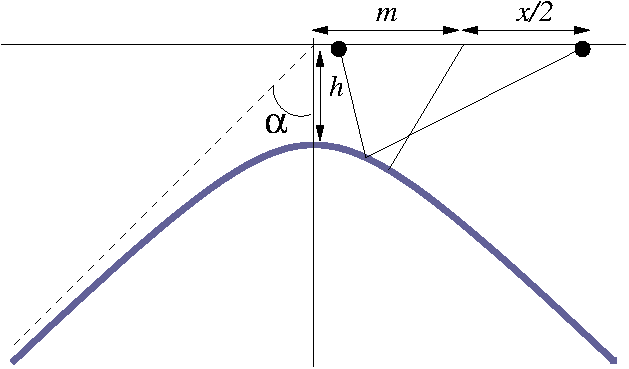
\includegraphics[width=0.450\textwidth,height=0.330\textwidth]{hyper/Fig/hyper}
%    \label{fig:hyper}}
%   \caption{Synthetic data example for testing. (a) Clean data. (b) Noisy data.}
%   \label{fig:hyper-clean,hyper}
%\end{figure}


%\begin{figure}[htb!]
%  \centering
%  \subfigure[]{\includegraphics[width=0.450\textwidth,height=0.330\textwidth]{hyper/Fig/hyper-fxemd0}
%    \label{fig:hyper-fxemd0}}
%  \subfigure[]{\includegraphics[width=0.450\textwidth,height=0.330\textwidth]{hyper/Fig/hyper-fxemd-noise0}
%    \label{fig:hyper-fxemd-noise0}}
%  \subfigure[]{\includegraphics[width=0.450\textwidth,height=0.330\textwidth]{hyper/Fig/hyper-fxmssa0}
%    \label{fig:hyper-fxmssa0}}
%  \subfigure[]{\includegraphics[width=0.450\textwidth,height=0.330\textwidth]{hyper/Fig/hyper-fxmssa-noise0}
%    \label{fig:hyper-fxmssa-noise0}}
%  \subfigure[]{\includegraphics[width=0.450\textwidth,height=0.330\textwidth]{hyper/Fig/hyper-fxemdmssa0}
%    \label{fig:hyper-fxemdmssa0}}
%  \subfigure[]{\includegraphics[width=0.450\textwidth,height=0.330\textwidth]{hyper/Fig/hyper-fxemdmssa-noise0}
%    \label{fig:hyper-fxemdmssa-noise0}}
%   \caption{Comparison of denoising effects. (a) Denoised using $f-x$ EMD. (b)  Noise section corresponding to (a). (c) Denoised using $f-x$ \old{M}SSA. (d) Noise section corresponding to (b). (e) Denoised using the proposed selective hybrid approach.  (f) Noise section corresponding to (c). The frame boxes in (b) are the two selective hybrid processing windows. }
%   \label{fig:hyper-fxemd0,hyper-fxmssa0,hyper-fxemdmssa0,hyper-fxemd-noise0,hyper-fxmssa-noise0,hyper-fxemdmssa-noise0}
%\end{figure}

\inputdir{hyperoil}

\multiplot{2}{hyper-clean,hyper}{width=0.450\textwidth,height=0.330\textwidth}{Synthetic data example for testing. (a) Clean data. (b) Noisy data (SNR=3.439).}

\multiplot{6}{hyper-fxemd0,hyper-fxmssa0,hyper-fxemdmssa0,hyper-fxemd-noise0,hyper-fxmssa-noise0,hyper-fxemdmssa-noise0}{width=0.450\textwidth,height=0.330\textwidth}{Comparison of denoising effects. (a) Denoised using $f-x$ EMD (SNR=3.136). (b)  Noise section corresponding to (a). (c) Denoised using $f-x$ \old{M}SSA (SNR=3.899). (d) Noise section corresponding to (b). (e) Denoised using the proposed selective hybrid approach (SNR=5.334).  (f) Noise section corresponding to (c). The frame boxes in (b) are the two selective hybrid processing windows. }

\plot{hyper-traces}{width=\textwidth}{Amplitude comparison for the 15th trace of the hyperbolic example.}

\inputdir{field}

\plot{pp}{width=0.450\textwidth,height=0.330\textwidth}{Field data example for testing.}

\multiplot{6}{pp-fxemd,pp-fxemd-noise0,pp-fxmssa,pp-fxmssa-noise0,pp-fxemdmssa,pp-fxemdmssa-noise0}{width=0.450\textwidth,height=0.330\textwidth}{Comparison of denoising effects. (a) Denoised using $f-x$ EMD. (b)  Noise section corresponding to (a). (c) Denoised using $f-x$ \old{M}SSA. (d) Noise section corresponding to (b). (e) Denoised using the proposed selective hybrid approach.  (f) Noise section corresponding to (c). The frame box in (b) is the selective hybrid processing window. }

\multiplot{4}{pp-mssa-zoom,pp-emdmssa-zoom,pp-emd-zoom,pp-emdmssa-zoom1}{width=0.45\textwidth,height=0.5\textwidth}{
Comparison of zoomed sections. (a) \& (b): comparison for frame box A in Figure \ref{fig:pp-fxemd,pp-fxemd-noise0,pp-fxmssa,pp-fxmssa-noise0,pp-fxemdmssa,pp-fxemdmssa-noise0}. (c) \& (d): comparison for frame box B in Figure \ref{fig:pp-fxemd,pp-fxemd-noise0,pp-fxmssa,pp-fxmssa-noise0,pp-fxemdmssa,pp-fxemdmssa-noise0}.}


\new{
\section{Discussions}}
\new{
In this section, we would like to give some comments on the practical aspects of the applications of the proposed approach.}
\begin{enumerate}
\item \new{Currently, $f-x$ EMD can not be widely used in real seismic data processing because of two main reasons: (1) not efficient and (2) causing damage to dipping energy. For the efficiency issue, as modern computational power is increasing very fast and fortunately the $f-x$ EMD is implemented in frequency-space domain frequency by frequency, we can developing parallel version of $f-x$ EMD codes in order to make it run fast. We also want to clarify that with the incomplete EMD as proposed in \cite{yangkang20132}, the computational cost of $f-x$ EMD is actually not too heavy, especially when compared with EEMD and CEEMD, which are prohibitively unaffordable and are difficult for parallelizing. For the dipping-removal issue, we can solve it easily by using a hybrid $f-x$ EMD approaches, which is being discussed in the paper and also investigated a lot in the literature. }

\item \new{The proposed selective hybrid approach is designed specifically following the special property of seismic data. As we all know, the post-stack or post-migration seismic images mainly contain horizontal events. How to fully use the advantage of $f-x$ EMD in handling horizontal events and also deal with complex structure becomes the focus of the presented work. Instead of using a full hybrid $f-x$ EMD approach, which make sure no coherent dipping events are lost, we propose to use a selective hybrid strategy. The hybrid approach is only applied to those regions where complex structure exist, leaving other simple horizontal events processed only using $f-x$ EMD. The selective hybrid $f-x$ EMD can be applied in local processing windows, in which case an automatic approach for detecting complex structure should be developed, and can also be applied to the global window, where complex structures are manually picked out for processing with a variable hybrid processing window, such as the second example in this paper (even though it is a pre-stack test). The local selective hybrid approach is applicable to relatively bigger dataset and with relatively more complicated structures. The global selective hybrid approach is applicable to relatively smaller dataset and with relatively simpler structures. }

\item \new{A graphical user interface (GUI) can be developed to best utilize the proposed selective hybrid $f-x$ EMD. In the GUI software, the seismic data can be processed section by section. The $f-x$ EMD is applied to the whole dataset initially, then we can pick out different area in the graphical interface for hybrid denoising conveniently. The GUI approach can deal with any dataset with different complexities and do not need the automatic complex-structure detection algorithm.}

\item \new{The horizontal-preservation property mentioned in this paper does not mean \emph{strictly horizontal preservation}. Unlike 1D mean and median filters, $f-x$ EMD can also preserve useful reflections with small dip angle. Compared with KL or SVD transforms, the $f-x$ EMD can be much more adaptive, because the horizontal events mainly lay in the first 1$-$3 IMFs after EMD in the $f-x$ domain, however, the number of singular values corresponding to the useful horizontal reflections for KL or SVD transforms have a large range and thus is not convenient to chose. According to our experience, the performance for preserving horizontal events of $f-x$ EMD is also much better that that of KL or SVD transforms.}
\end{enumerate}

\section{Conclusions}
We have analyzed and demonstrated the horizontal-preservation and dipping-removal properties of $f-x$ EMD. \new{The ability of $f-x$ EMD to preserve horizontal events is very strong, however, it is very sensitive to dipping events. Even after removing many IMFs in the $f-x$ domain, the horizontal events can still be preserved. However, even removing one or two IMFs in the $f-x$ domain, the dipping events can be totally removed.} In order to solve the problem of $f-x$ EMD in dealing with complex structure that contains dipping events \new{and at the same to improve the accuracy for a selected dipping-events retriever}, we have proposed a novel and general hybrid denoising framework, which fully utilizes the horizontal-preservation capability of $f-x$ EMD in dealing with non-stationary seismic data and the dipping-preservation capability of the selected dipping-events retriever. As a tutorial, $f-x$ \old{M}SSA is selected to be combined with $f-x$ EMD in this paper. 

A selective hybrid strategy is also proposed to maximize the effectiveness of $f-x$ EMD and the processing efficiency. The current selective hybrid approach is based on manually selected processing windows, which is inconvenient for implementation when seismic profile is over complicated. An automatic way to detect the specific windows containing complex structure and to implement the selective hybrid denoising approach is the topic of current research.  From the synthetic and field data examples, it's obvious that, the proposed selective hybrid approach can effectively obtain better results compared with both $f-x$ EMD and the selected dipping-events retriever.

\section{Acknowledgments} 
We thank Sergey Fomel, Ryan Swindeman, Jitao Ma, Mauricio Sacchi, Karl Schleicher, and Josef Paffenholz for helpful discussions. \new{We also thank three anonymous reviewers for constructive suggestions that help make the manuscript better.} This paper and all the figures are prepared with the Madagascar software package, which is an open-source research environment for reproducible computational experiments \cite[]{mada2013}. Thus, we are grateful for its developers for providing such convenience. 
\bibliographystyle{seg}
\bibliography{emdnoise}






